% !TeX program = lualatex
% !TeX root = main.tex
% Template de Relatório de Estágio - Normas ABNT
\documentclass[12pt,a4paper]{article}

% Pacotes essenciais
\usepackage[brazilian]{babel}
\usepackage{fontspec}
%\setmainfont{Arial}
\usepackage{geometry}
\usepackage{setspace}
\usepackage{graphicx}
\usepackage{tikz}
\usepackage[hidelinks,hypertexnames=false]{hyperref}
\usepackage{titlesec}
\usepackage{tocloft}
\usepackage{fancyhdr}
\usepackage{lmodern}
\usepackage{svg}


\newcommand{\Name}{Gabriel Cunha Marchetti}
\newcommand{\University}{UNICAMP - Universidade Estadual de Campinas.}
\newcommand{\Lnls}{LABORATÓRIO NACIONAL DE LUZ SÍNCROTRON}
\newcommand{\TituloTrabalho}{Título do Trabalho}
\newcommand{\CNB}{CARNAUBA}
\newcommand{\Orientador}{Nome do orientador}
\newcommand{\Relator}{Nome do relator}


% Configurações ABNT
\geometry{
    a4paper,
    left=3cm,
    right=2cm,
    top=3cm,
    bottom=2cm
}

% Espaçamento 1,5
\setstretch{1.5}

% Configuração de parágrafos
\setlength{\parindent}{1.25cm}
\setlength{\parskip}{0pt}

% Citações ABNT - usando abnTeX2
\usepackage[alf,abnt-etal-list=0,abnt-etal-text=it]{abntex2cite}

% Formatação de títulos
\titleformat{\section}
{\normalfont\fontsize{18}{15}\bfseries}
{\thesection}{1em}{}

\titleformat{\subsection}
{\normalfont\fontsize{12}{15}\bfseries\raggedright}
{\thesubsection}{1em}{}

% Cabeçalho e rodapé
\pagestyle{fancy}
\fancyhf{} % Limpa cabeçalho e rodapé
\fancyhead[L]{
\includegraphics[height=1.5cm]{imagens/cnpem.png}} % Logo no topo esquerdo
\fancyfoot[R]{\thepage} % Número da página no rodapé direito
\renewcommand{\headrulewidth}{0pt} % Remove linha do cabeçalho
\renewcommand{\footrulewidth}{0pt} % Remove linha do rodapé
\setlength{\headheight}{2cm} % Altura do cabeçalho para acomodar a imagem

% Sumário
\renewcommand{\contentsname}{Sumário}
\renewcommand{\cftsecleader}{\cftdotfill{\cftdotsep}}

% Início do documento
\begin{document}

% ============= CAPA =============
\begin{titlepage}
    \vspace*{-4cm}
    \hspace*{-2cm}
\includegraphics[height=1.5cm]{imagens/cnpem.png}
    \vspace{1cm}
    \begin{center}
        \fontsize{14}{17}\selectfont
        \textbf{\Lnls}
        
        \vspace{4cm} 
        
        \textbf{\Name}
        
        \vfill 
        
        \textbf{\TituloTrabalho}
        
        \vfill 
        
        \textbf{CAMPINAS -- SP}\\
        \textbf{2026}
    \end{center}
\end{titlepage}

% ============= FOLHA DE ROSTO =============
\begin{titlepage}
    \vspace*{-4cm}
    \hspace*{-2cm}
\includegraphics[height=1.5cm]{imagens/cnpem.png}
    \vspace{1cm}
    \begin{center}
        \fontsize{14}{17}\selectfont
        \textbf{\Lnls}
        
        \vspace{4cm}
        
        \textbf{\Name}
        
        \vspace{3cm}
        
        \textbf{\TituloTrabalho}
        
        \vspace{3cm}
    \end{center}
    
    \setlength{\fboxsep}{15pt}
    \setlength{\fboxrule}{0.8pt}
    \begin{flushright}
        \fbox{
            \begin{minipage}{6cm}
                \fontsize{11}{13}\selectfont
                Estágio realizado junto ao \CNB\ para o \Lnls, sob a orientação de \Orientador\ -- desde janeiro de 2026.
            \end{minipage}
        }
    \end{flushright}
    
    \vspace{1cm}
    
    \begin{flushright}
    \parbox{8cm}{
        \centering \Orientador\\[-0.4cm]
        \rule{\linewidth}{0.4pt}\\
        \centering Nome do Orientador
    }
    
    \vspace{1cm}

    \parbox{8cm}{
        \centering \Relator\\[-0.4cm] % Diminui o espaço antes da linha
        \rule{\linewidth}{0.4pt}\\
        \centering Nome do Relator
    }
    \end{flushright}

    \begin{center}
        \vfill
        \textbf{CAMPINAS -- SP}\\
        \textbf{2026}
    \end{center}
    
\end{titlepage}

% ============= SUMÁRIO =============
\tableofcontents
\newpage

% ============= CORPO DO TEXTO =============
\fontsize{11}{16.5}\selectfont % Define fonte 11pt com espaçamento 1.5

\phantomsection
\section*{Introdução}
\addcontentsline{toc}{section}{Introdução}

As linhas de luz síncrotron são estações experimentais que utilizam a radiação síncrotron para realizar investigações científicas em diversas áreas do conhecimento, como biologia, química, ciência dos materiais e geociências \cite{xiao_chao_1}. 
A incidência de raios-X de alto brilho sobre os materiais permite a obtenção de informações detalhadas sobre suas estruturas internas, tanto em escala atômica ou molecular.

O \Lnls\ é um exemplo de instalação que abriga linhas de luz síncrotron, oferecendo infraestrutura avançada, como controle de estabilidade do feixe e um arranjo óptico sofisticado \cite{liu_lin_1}, para a realização de experimentos científicos de ponta, como XRF (\textit{X-ray Fluorescence}) e XANES (\textit{X-ray Absorption Near Edge Structure}) \cite{lnlslinhas}.
Sendo uma dessas linhas a linha de luz \CNB\, onde são realizados experimentos que demandam alta precisão (na ordem nanométrica) na análise estrutural de materiais. 

Contudo, essa alta precisão requer diversos cuidados de metrologia e uma infraestrutura adequada, para além da estrutura do anel, para garantir a confiabilidade dos resultados obtidos. 
Sendo inicialmente proposta uma metodologia para caracterização do feixe através de imagens de absorção de raios-X, XAS (\textit{X-ray Absorption Spectroscopy}), e outras técnicas complementares.

Esse plano de caracterização do feixe é conhecido como cáustica e envolve uma obtenção do perfil espacial do feixe em diferentes condições de operação para avaliar possíveis relações de causa-efeito dentro de ajustes.
Como, por exemplo, a influência de elementos ópticos no perfil do feixe, variações na intensidade e possíveis distorções causadas, como astigmatismo do feixe. 

Tal resultado é numericamente quantificado como o foco da linha de luz. Esse parâmetro é essencial para garantir a qualidade e a precisão dos experimentos realizados, permitindo ajustes finos na configuração óptica e na posição dos elementos experimentais.
Além disso, possui outra característica prática, experimentos podem demandar diferentes níveis de foco, havendo até mesmo experimentos que necessitam de focos na ordem dos micrômetros, uma escala muito menor que a ordem nanométrica mencionada anteriormente.

Essa variação na necessidade de foco implica que a linha de luz deve ser capaz de ajustar seu perfil de feixe de acordo com os requisitos específicos de cada experimento, garantindo assim a flexibilidade e a precisão necessárias para diferentes tipos de investigações científicas.



\newpage
\phantomsection
\section*{Objetivo}
\addcontentsline{toc}{section}{Objetivo}

O problema abordado nesse projeto envolve a caracterização e estudo de um método de cáustica para a linha de luz \CNB. 
Compreende dentro desse contexto uma experimentação com âmparo teórico, buscando validar os resultados obtidos e compreender os fenômenos observados de maneira mais aprofundada.
Mas ainda obter resultados empíricos que possam corroborar as previsões teóricas, garantindo assim a robustez e a confiabilidade das conclusões do estudo.

A obtenção de um método de cáustica bem definido é extremamente benéfico para os operadores da linha de luz, uma vez que se trata de um processo manual e qualitativo. 
Dessa forma, as análises ficam inconsistentes entre si, dificultando a comparação de resultados e a reprodutibilidade dos experimentos.
Além de que há um ganho de tempo para outras atividades.

Veja que seu desenvolvimento está em de acordo com a automatização dos sistemas de controle e análise da linha de luz através do \textit{framework} de operação EPICS aliado à biblioteca \textit{Bluesky}, mais adiante entraremos em detalhe sobre esses sistemas.

O resultado pretendido dentro desse projeto é um plano de cáustica que capte os dados de forma automatizada e que possa ser analisado por um script ou programa de interpretação e processamento de dados. 

\newpage
\phantomsection
\section*{Método}
\addcontentsline{toc}{section}{Método}

\phantomsection
\subsection*{Descrição dos fenômenos observados.}
\addcontentsline{toc}{subsection}{Descrição dos fenômenos observados.}

Raios-X são radiações eletromagnéticas de alta energia, capazes de atravessar materiais opacos à luz visível. Eles possuem comprimentos de onda muito curtos, geralmente na faixa de 0,01 a 10 nanômetros, o que lhes confere grande poder de penetração e capacidade de interação com a matéria em nível atômico.
Nesse regime, os raios-X são absorvidos pela matéria através do efeito foto-elétrico, nesse processo um fóton incidente transfere toda a sua energia a um elétron, que é então ejetado do átomo, resultando na ionização da matéria.

Para que um nível eletrônico específico seja afetado pela radiação dos raios-X, a energia do fóton incidente deve ser suficiente para superar a energia de ligação do elétron nesse nível. Caso contrário, o fóton não conseguirá ejetar o elétron, e a interação não resultará em ionização \cite{matthew_newville}. 
O processo é exemplificado na Figura \ref{efeito-fotoeletrico}.

\begin{figure}[h]
    \centering
        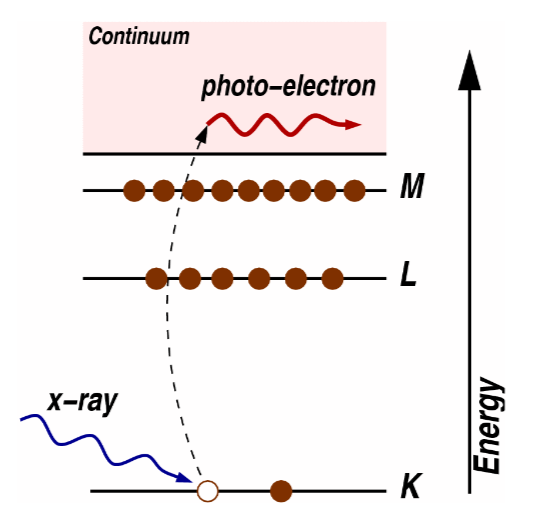
\includegraphics[width=0.5\linewidth]{imagens/efeito-fotoeletrico.png}
    \caption{Efeito fotoelétrico - um fóton incidente transfere sua energia a um elétron, que é ejetado do átomo. Imagem extraída de \cite{matthew_newville}}
    \label{efeito-fotoeletrico}
\end{figure}

Contudo, esse fenômeno não é exclusivo na incidência de raios-X sobre uma amostra. Mas, para esse trabalho se trata do fenômeno em destaque para desenvolvimento do método de cáustica.

Os outros fenômenos que podem ocorrer são: 
\begin{itemize}
    \item Espalhamento Elástico (Rayleigh): um fóton incidente colide com um elétron, transferindo parte de sua energia e mudando sua direção. 
    \item Espalhamento Inelástico (Compton): o fóton é espalhado elasticamente pela matéria, sem perda de energia.
    \item Transmissão sem interação: O fóton atravessa a amostra sem ser absorvido ou espalhado. Permite medir a atenuação e formar imagens por transmissão.
    \item Fluorescência de raios-X: um fóton incidente é absorvido por um átomo, que em seguida emite um fóton de menor energia característico do elemento.
    \item Luminescência: emissão de luz por um material após absorver radiação, podendo ocorrer em diferentes comprimentos de onda dependendo do material.
\end{itemize}

Veja que essa é uma listagem dos fenômenos que podem ocorrer quando a radiação interage com a matéria, como ilustrada na Figura \ref{exemplos-de-interacao-materia}. 
Apesar de não haver muita relevância para o desenvolvimento do método de cáustica, sua compreensão é importante para o entendimento da linha de luz \CNB e sobretudo sobre algumas limitações do método.

\begin{figure}[h]
    \centering
        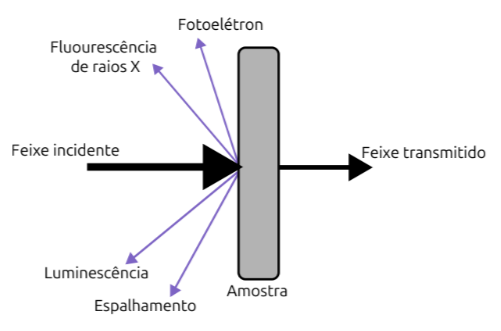
\includegraphics[width=0.6\linewidth]{imagens/radiacao-materia.png}
    \caption{Ilustração dos fenômenos que podem ocorrer quando a radiação interage com a matéria. Imagem extraída de \cite{murilo_theodoro}}
    \label{exemplos-de-interacao-materia}
\end{figure}

Através da equação de \textbf{Beer-Lambert}. É possível calcular a atenuação da radiação ao atravessar a amostra, relacionando a intensidade incidente com a intensidade transmitida e a espessura do material.

\begin{equation}
    I(E) = I_0(E) \cdot \exp\left[-\mu(E) \cdot t\right]
\end{equation}

Sendo que $I(E)$ é a intensidade transmitida, $I_0(E)$ é a intensidade incidente, $\mu(E)$ é o coeficiente de absorção linear e $t$ é a espessura da amostra.

A Figura~\ref{fig:atenuacao-amostra} ilustra a redução da intensidade ao atravessar a amostra, sendo $I_1(E) \equiv I(E)$ a intensidade transmitida.

\begin{figure}[htbp]
    \centering
    \begin{tikzpicture}[x=1cm,y=1cm,>=stealth,font=\small]
        % Amostra e feixes: a espessura das setas representa a intensidade.
        \filldraw[fill=gray!15,draw=gray!70] (4,0) rectangle (8,2.4);
        \node at (6,2.75) {Amostra: $\mu(E)$};
        \draw[->,blue!70!black,line width=3pt] (0.4,1.2) -- (3.8,1.2);
        \node[align=center] at (2.1,2.1) {$I_0(E)$\\Intensidade incidente};
        \draw[->,blue!70!black,line width=0.9pt] (8.2,1.2) -- (11.6,1.2);
        \node[align=center] at (9.9,2.1) {$I_1(E)<I_0(E)$\\Intensidade transmitida};
        \draw[<->] (4,-0.35) -- node[below] {Espessura $t$} (8,-0.35);
        % Perfil esquemático do decaimento exponencial dentro da amostra.
        \fill[gray!10] (4,-4.5) rectangle (8,-1.35);
        \draw[->] (0.4,-4.5) -- (11.6,-4.5) node[below] {Posição $x$};
        \draw[->] (0.7,-4.5) -- (0.7,-1.25) node[above] {Intensidade};
        \draw[dashed,gray] (4,0) -- (4,-4.5);
        \draw[dashed,gray] (8,0) -- (8,-4.5);
        \draw[blue!70!black,thick] (0.7,-1.8) -- (4,-1.8);
        \draw[blue!70!black,thick,domain=4:8,samples=60]
            plot (\x,{-4.5+2.7*exp(-0.35*(\x-4))});
        \draw[blue!70!black,thick] (8,-3.8342) -- (11,-3.8342);
        \node[above] at (2.3,-1.8) {$I_0$};
        \node[above] at (9.6,-3.8342) {$I_1=I_0e^{-\mu t}$};
        \node[below] at (4,-4.5) {$0$};
        \node[below] at (8,-4.5) {$t$};
    \end{tikzpicture}
    \caption{Atenuação da radiação ao atravessar uma amostra de espessura $t$. A intensidade decai exponencialmente no interior do material, de $I_0$ para $I_1$, conforme a lei de Beer--Lambert. Diagrama esquemático, sem escala.}
    \label{fig:atenuacao-amostra}
\end{figure}

Dentro do arranjo experimental é possível utilizar fotodiodos para medição tanto de $I(E)$ quanto para $I_0(E)$, enquanto que $t$ é facilmente medido diretamente com instrumentos de medição de espessura, como paquímetros ou através de um método de processamento das amostras.
Dessa forma, teremos que a equação se transforma em:

\begin{equation}
    \mu(E) = -\frac{1}{t} \ln\left[\frac{I(E)}{I_0(E)}\right] = \frac{1}{t} \ln\left[\frac{I_0(E)}{I(E)}\right] = \frac{1}{t} \ln\left[\frac{I_0}{I}(E)\right]
    \label{eq:absorption-beer-lambert}
\end{equation}

A partir dessa equação é possível fazer uma curva de absorção característica dos materiais analisados.

\begin{figure}[h]
    \centering
\        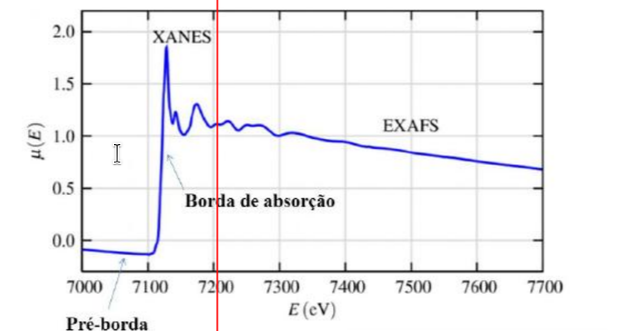
\includegraphics[width=0.6\linewidth]{imagens/curva-absorcao.png}
    \caption{Exemplo de curva de absorção característica de um material. Imagem extraída dos slides de aula de \href{https://portal.edat.unicamp.br/perfil?origem=&docente=328368&sigla_unidade=&nome_unidade=&nome_programa=}{VERÔNICA TEIXEIRA}}
    \label{curva-absorcao}
\end{figure}

Sendo que três áreas são característica do espectro de absorção: a Pré-borda, XANES (X-ray Absorption Near Edge Structure) e EXAFS (Extended X-ray Absorption Fine Structure), como exemplificado na Figura \ref{curva-absorcao}.

\textbf{Pré-Borda}: É a região do espectro de absorção que ocorre antes do pico de absorção principal. Nessa região, a absorção é relativamente baixa e geralmente não apresenta estruturas finas. 

\textbf{XANES}: É a região caracterizada pela aumento súbido da absorção próximo ao pico de absorção principal. Nessa região, podem ser observadas estruturas finas que fornecem informações sobre o estado de oxidação, coordenação e estado de \textit{spin} do elemento observado.

\textbf{EXAFS}: É a região do espectro de absorção que ocorre após o pico de absorção principal. Nessa região, a absorção apresenta oscilações finas que fornecem informações sobre a distância e o número de átomos vizinhos ao elemento absorvedor.

Além disso, há a relação do \textbf{XAS} com a \textbf{XRF}(\textit{X-ray Fluorescence}), que é uma técnica complementar utilizada para determinar a composição elementar de uma amostra \cite{murilo_theodoro}. 
Enquanto o \textbf{XAS} fornece informações sobre o estado químico e a estrutura local ao redor de um elemento específico, a \textbf{XRF} permite identificar e quantificar os elementos presentes na amostra.
Dessa forma, os seguintes métodos desenvolvidos dentro desse projeto também podem ser utilizados para imagens geradas a partir de técnicas de imageamento através de fluorescência de raios-X, com seus devidos ajustes. 
A equação \ref{eq:XAS-XRF-relation} demonstra essa relação e pode ser utilizada para gerar imagens possíveis de serem utilizadas para a execução do método.
Uma questão levantada durante o desenvolvimento do método até questionou se devido ao maior nível de precisão desses detectores de fluorescência haveria ganho na caracterização do feixe,
contudo não entramos em maiores detalhes, pois vários experimentos utilizar o método proposto pela equação \ref{eq:absorption-beer-lambert}.

\begin{equation}
    I_{XAS}(E) = \int_{E} I_{XRF}(E', h\omega) dE'
    \label{eq:XAS-XRF-relation}
\end{equation}

\phantomsection
\subsection*{Descrição da linha de luz}
\addcontentsline{toc}{subsection}{Descrição da linha de luz}

Diferente de dispositivos de espectroscopia de luz visível, infra-vermelho e micro-ondas, não há um aparato comercial que consiga reproduzir de forma completa os experimentos de espectroscopia de absorção de raios-X.
Dentro desse contexto vem a construção de linhas de luz que possibilitam realizar experimentos (como \textbf{XAS}), como a linha de luz \CNB.

\begin{figure}[h]
    \centering
        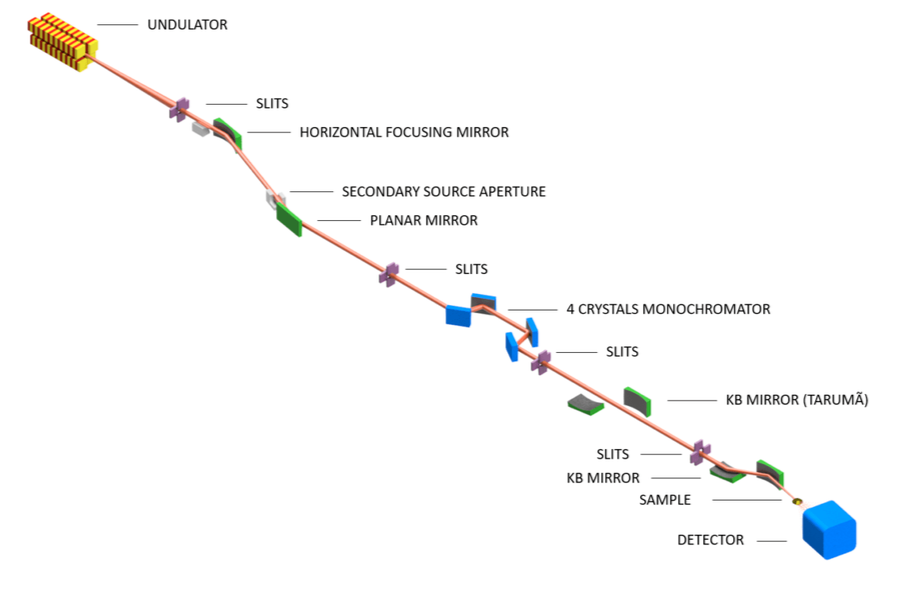
\includegraphics[width=0.65\linewidth]{imagens/esquematico_carnauba.png}
    \caption{Esquemático da linha de luz \CNB. Imagem extraída de \cite{lnlslinhas}}
    \label{esquematico_carnauba}
\end{figure}

O esquemático da linha de luz \CNB\ é apresentado na Figura \ref{esquematico_carnauba}. Ele ilustra os principais componentes e a disposição do aparato experimental.

Vamos começar pela definição desses componentes da linha de luz \CNB\ e suas funções. 
O Ondulador é uma estrutura magnética composta por diversos imãs de polaridade invertida colocados sequencialmente na trajetória do feixe.
Essa disposição faz com que o feixe de elétrons sofra uma oscilação periódica, resultando na emissão de radiação síncrotron altamente colimada e intensa \cite{esrf_1}. O exemplo de um ondulador é apresentado na Figura \ref{ondulador}, sendo representado o efeito de adição de harmônicos.

\begin{figure}[h]
    \centering
        \includesvg[width=0.6\linewidth]{imagens/ondulator-exemplo.svg}
    \caption{Exemplo de ondulador utilizado em linhas de luz de síncrotron. Imagem extraída de \href{https://upload.wikimedia.org/wikipedia/commons/f/f3/Undulator.svg?utm_source=en.wikipedia.org&utm_campaign=index&utm_content=original}{Wikipedia}}
    \label{ondulador}
\end{figure}

Além disso, há o controle de otimização da energia emitida pelo Ondulador, medida através de eV, através de um sistema de ajuste da distância entre os ímãs, permitindo variar a intensidade e/ou a frequência da radiação emitida, esse parâmetro é referenciado como \textbf{GAP}.

Veja que o ajuste do \textbf{GAP} é o que permite otimizar a energia em equações como a equação \ref{eq:absorption-beer-lambert}

Enquanto isso, as fendas (\textit{slits}) são utilizadas para definir a geometria do feixe de luz, controlando sua largura e altura, e garantindo que apenas a porção desejada do feixe passe para a próxima etapa.
Como efeito imediato de seu fechamento, ocorre a redução do fluxo de fótons, que pode ser vantajosa para experimentos com amostras biológicas e suscetíveis à radiação, enquanto a abertura das fendas permite um maior fluxo de fótons, adequado para experimentos que requerem maior intensidade de radiação e maior contraste.

Na sequência óptica da linha \CNB, o primeiro espelho, denominado \textbf{M1} (\textit{Mirror-1}), focaliza o feixe no plano da fonte secundária. Nesse plano, a \textbf{SSA}(\textit{Secondary Source Aperture}) delimita a região transmitida e define o tamanho efetivo da fonte vista pelos componentes seguintes (um comportamento muito similar ao das fendas). Sua abertura permite estabelecer um compromisso entre fluxo de fótons e coerência espacial. O segundo espelho, denominado \textbf{M2} (\textit{Mirror-2}), realiza a deflexão horizontal do feixe, direcionando-o ao longo do percurso óptico \cite{lnlscarnaubaoptica}, \cite{nanomax2021}.

As vistas frontal e traseira do conjunto do \textbf{M1} são apresentadas na Figura~\ref{fig:m1-hutch-a}. 
Uma imagem do espelho \textbf{M2} foi omitida, uma vez que é similar ao \textbf{M1}.

\begin{figure}[htbp]
    \centering
    \begin{minipage}[t]{0.48\linewidth}
        \centering
        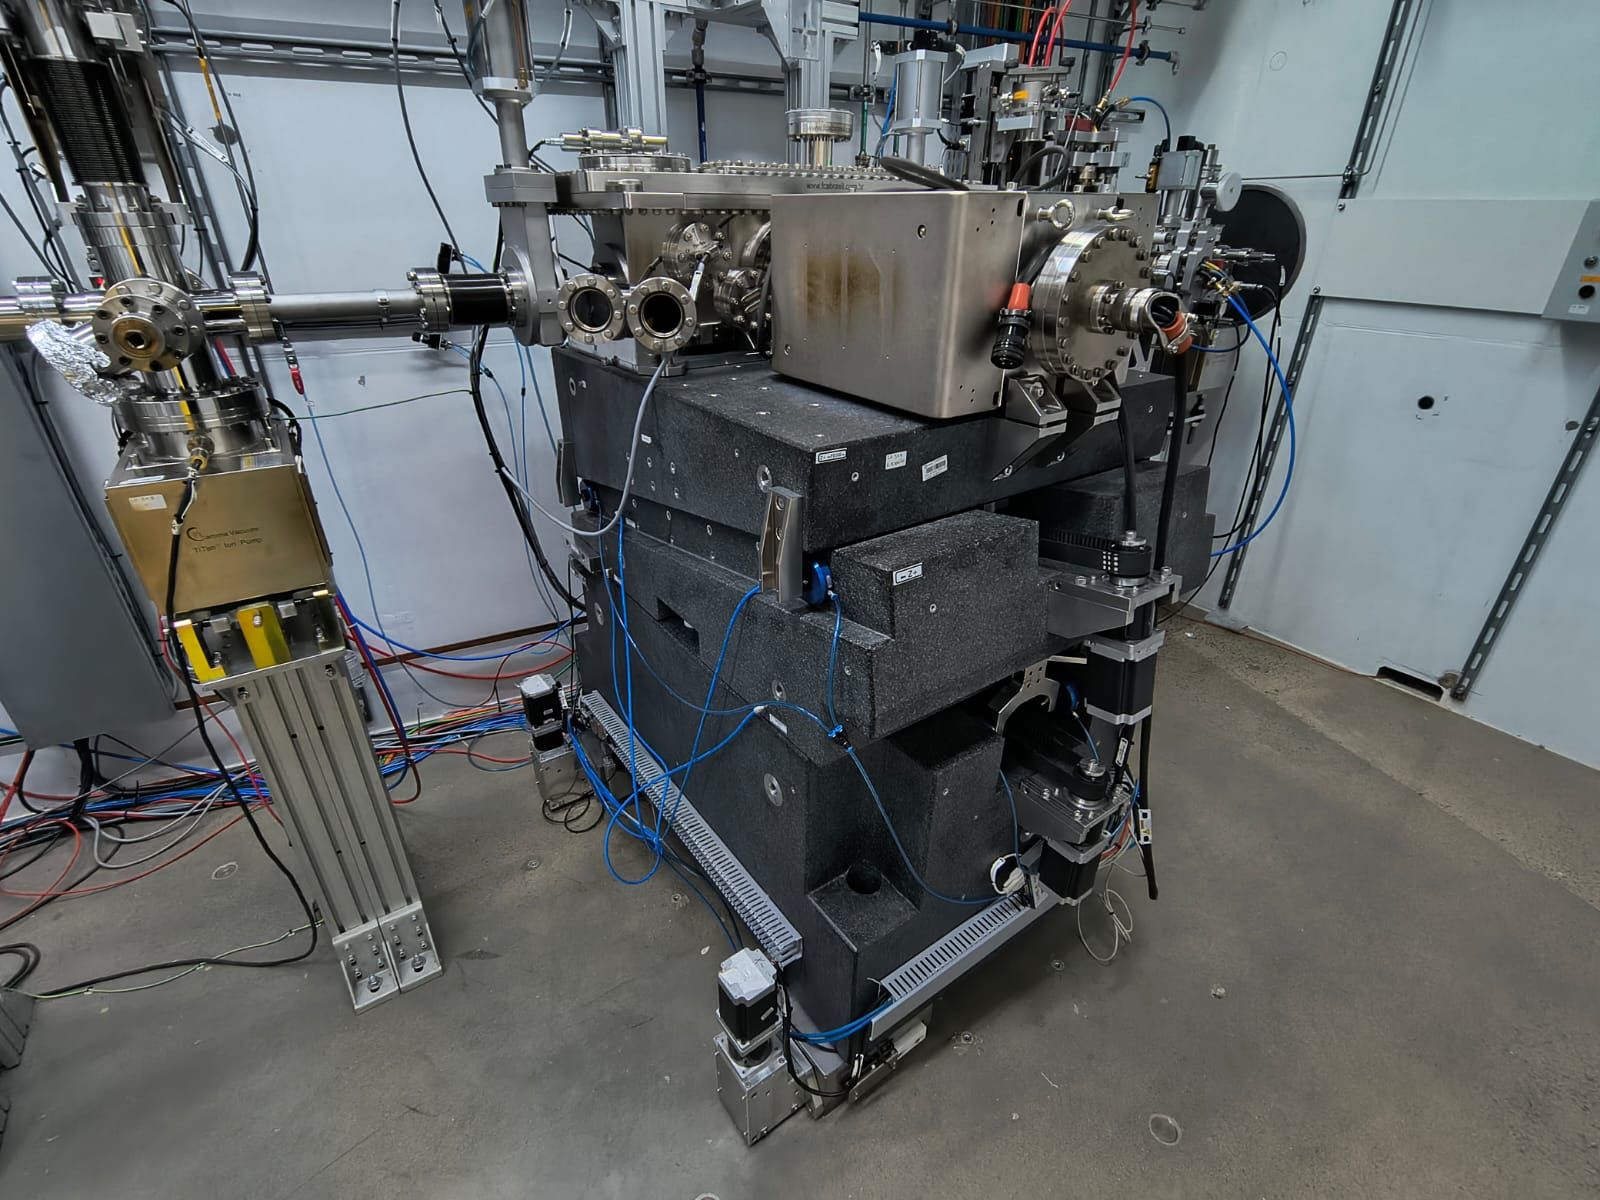
\includegraphics[width=\linewidth]{imagens/m1-hutchA-front.jpeg}
        \par\small (a) Vista frontal.
    \end{minipage}\hfill
    \begin{minipage}[t]{0.48\linewidth}
        \centering
        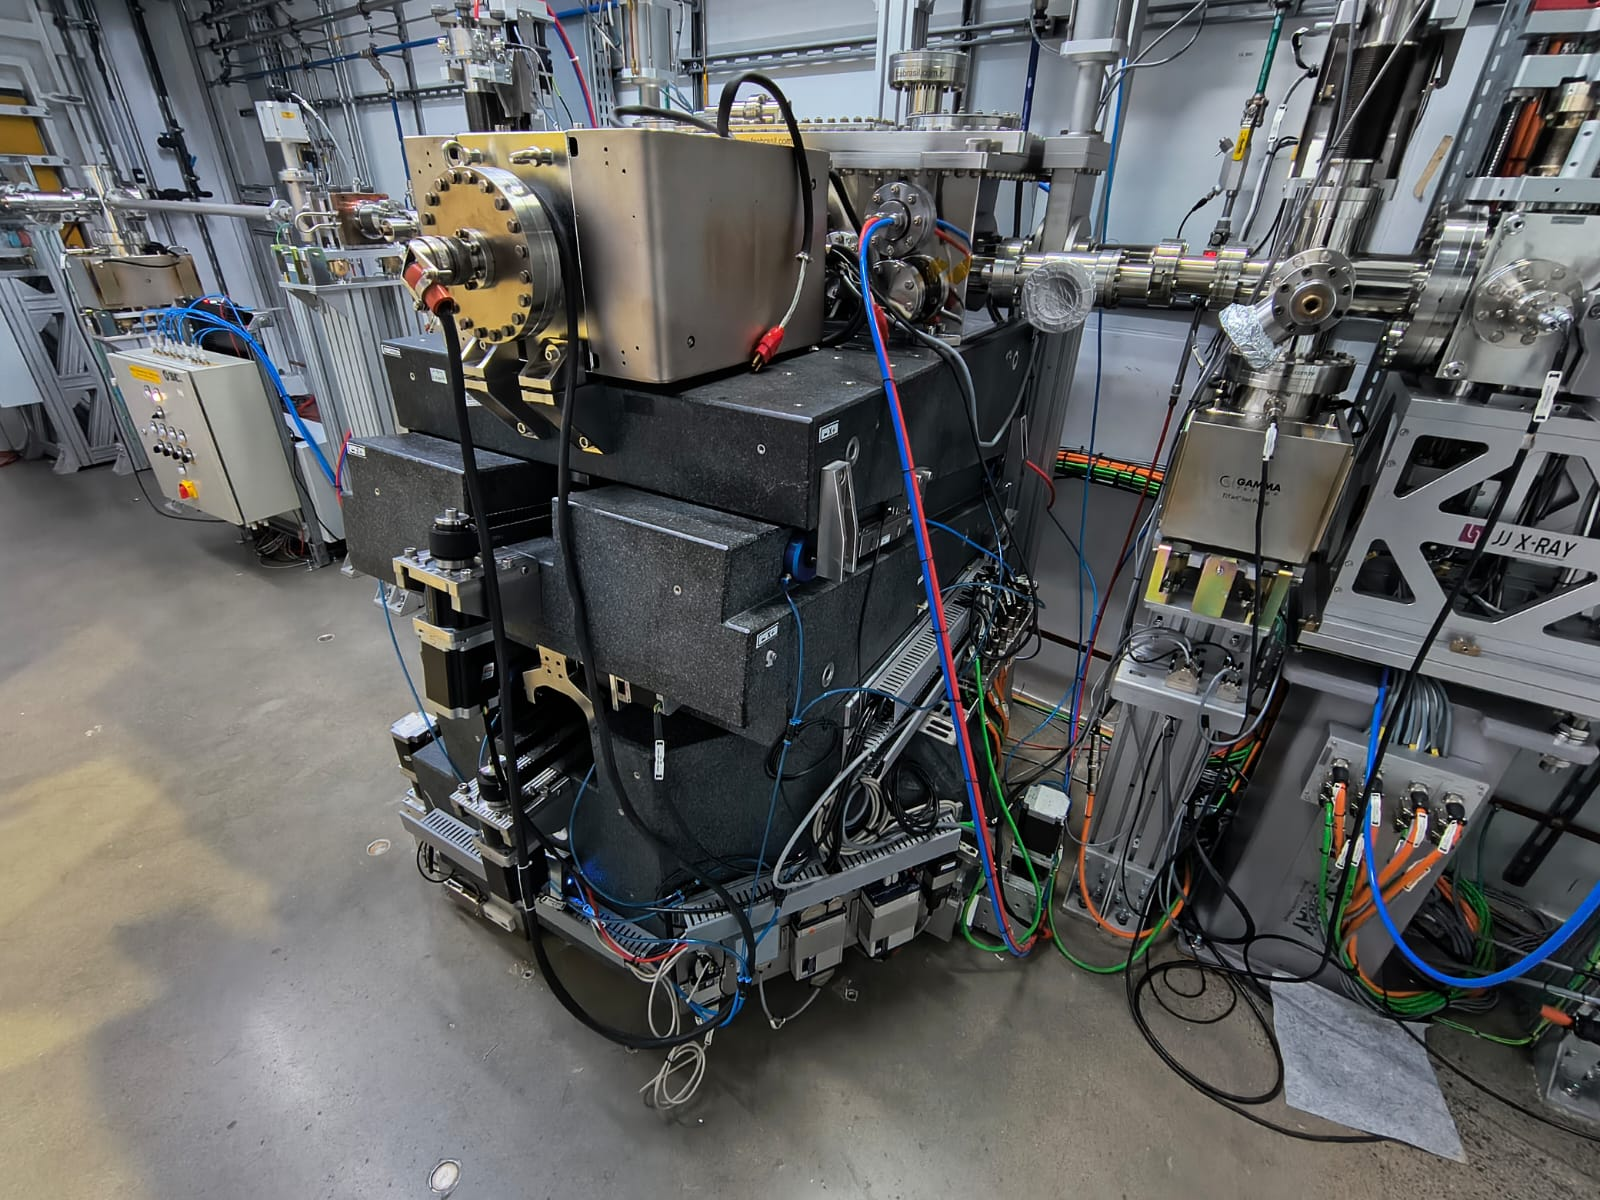
\includegraphics[width=\linewidth]{imagens/m1-hutchA-back.jpeg}
        \par\small (b) Vista traseira.
    \end{minipage}
    \caption{Conjunto do primeiro espelho (M1) na cabana experimental: (a) vista frontal e (b) vista traseira.}
    \label{fig:m1-hutch-a}
\end{figure}

A seleção da energia utilizada no experimento é realizada pelo \textbf{monocromador de quatro cristais (4CM)}, que utiliza reflexões em cristais de silício para selecionar uma faixa estreita de energias. Essa seleção obedece à condição de Bragg, relacionando o comprimento de onda ao espaçamento entre os planos cristalinos e ao ângulo de incidência. Assim, enquanto o \textbf{GAP} do ondulador ajusta o espectro disponível na fonte, o monocromador seleciona a energia incidente na amostra e permite sua varredura durante a aquisição de espectros de \textbf{XAS} \cite{lnlscarnaubaoptica}.
Veja que o \textbf{monocromador} é essencial para filtrar os comprimentos de onda indesejados, uma vez que os onduladores emitem radiação em múltiplos harmônicos que podem prejudicar a análise experimetal.

O conjunto do \textbf{monocromador de quatro cristais (4CM)} é apresentado na Figura~\ref{fig:4cm-hutch-c}.

\begin{figure}[htbp]
    \centering
    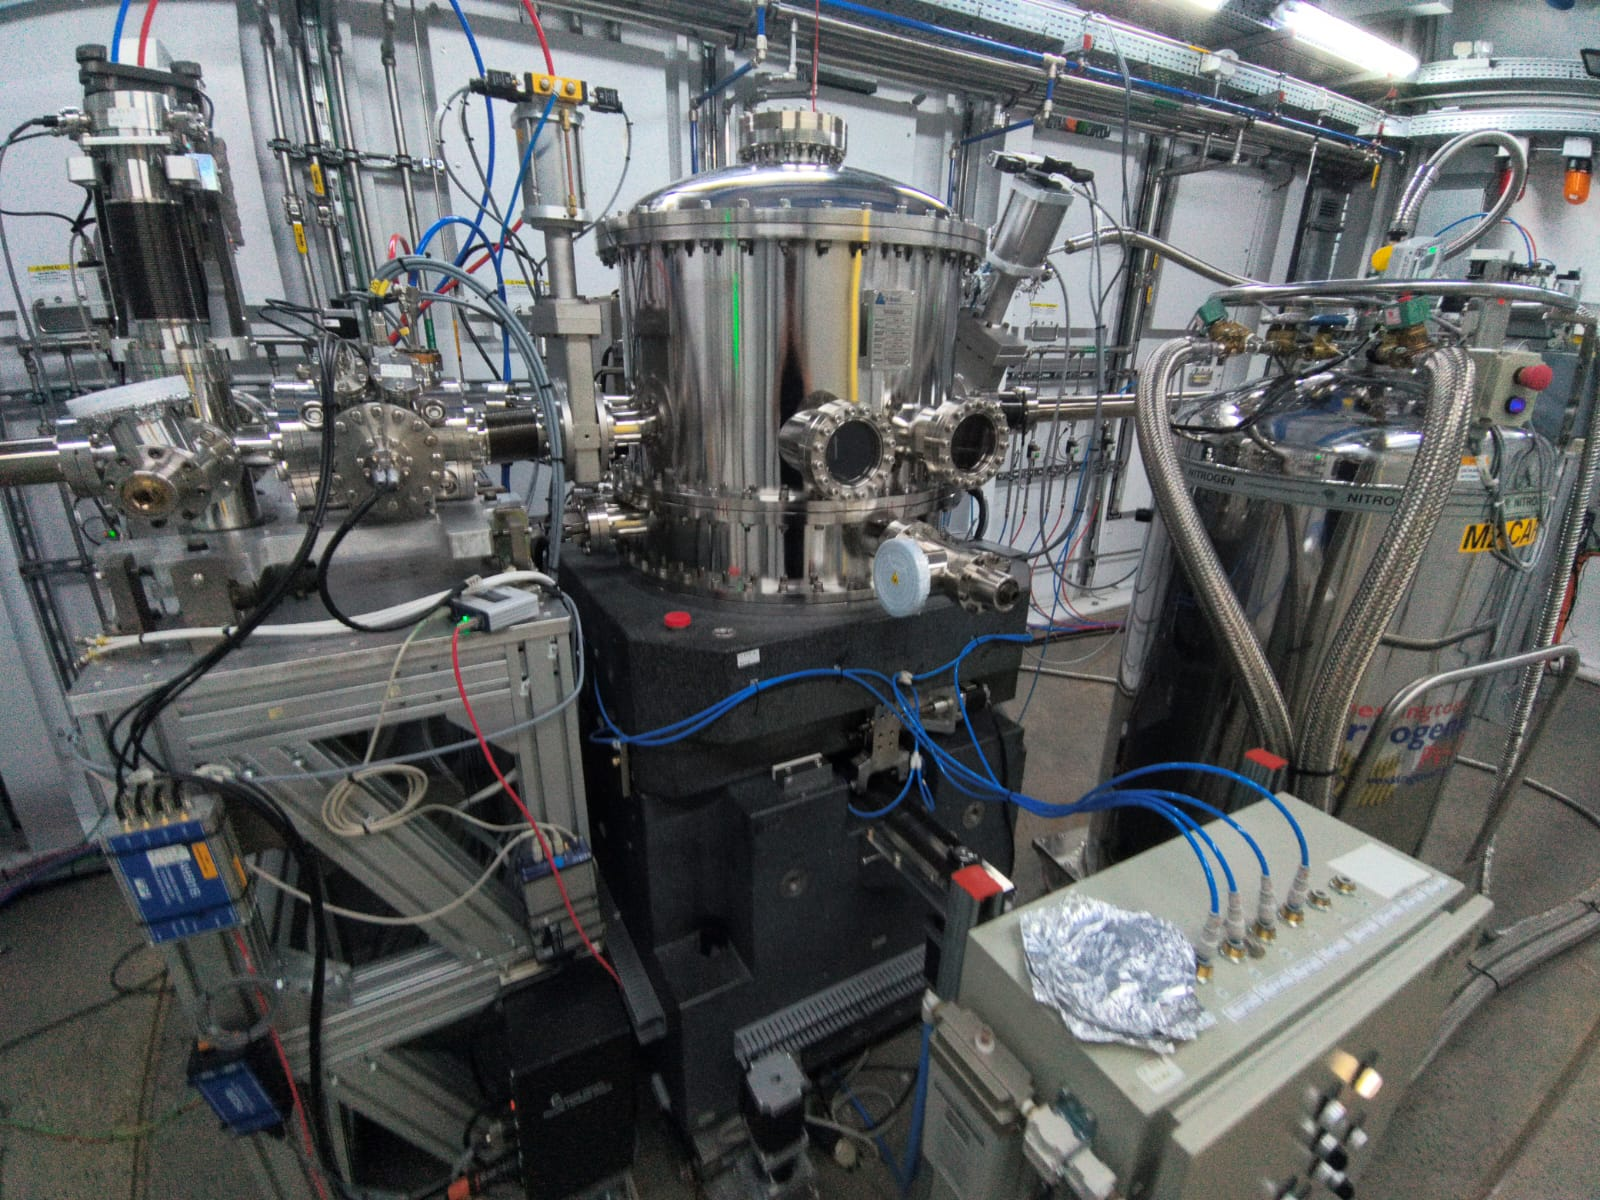
\includegraphics[width=0.75\linewidth]{imagens/4cm-hutchC.jpeg}
    \caption{Conjunto do monocromador de quatro cristais (4CM) na cabana experimental.}
    \label{fig:4cm-hutch-c}
\end{figure}

Próximo à amostra, os espelhos \textbf{Kirkpatrick--Baez (KB)} realizam a focalização final. O par possui um espelho responsável pela focalização vertical e outro pela horizontal, concentrando o feixe em uma pequena região da amostra. Esse arranjo está presente nas estações TARUMÃ e SAPOTI e permite realizar medidas espacialmente resolvidas \cite{lnlscarnaubaoptica}.

O arranjo dos espelhos \textbf{Kirkpatrick--Baez (KB)} é ilustrado na Figura~\ref{fig:kb-diagram}.

\begin{figure}[htbp]
    \centering
    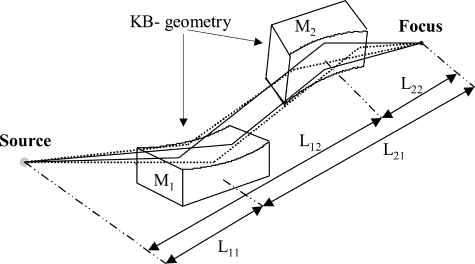
\includegraphics[width=0.75\linewidth]{imagens/kb-diagram.png}
    \caption{Diagrama do arranjo de espelhos Kirkpatrick--Baez (KB). Imagem extraída de \href{https://www.j-tec.co.jp/english/optical/optical-products/kb-mirror/}{JTEC Corporation}.}
    \label{fig:kb-diagram}
\end{figure}

Desse modo, a óptica prepara a energia e a distribuição espacial da radiação incidente. A formação de mapas ocorre pela varredura da amostra em relação ao feixe focalizado e pelo registro do sinal em cada posição; ao repetir esse procedimento para diferentes energias, podem ser obtidos mapas espectroscópicos de absorção \cite{lnlscarnaubaoptica} como os mostrados em Figura \ref{curva-absorcao}.

\phantomsection
\subsection*{Descrição das estações experimentais}
\addcontentsline{toc}{subsection}{descrição das estações experimentais}

Dentro da linha de luz \CNB\ existem duas estações experimentais, sendo elas a TARUMÃ e a SAPOTI. 
A primeira providencia um tamanho de feixe submicrométrico e ambiente de amostras variável, enquanto a SAPOTI possui tamanho de feixe nanométrico e ambiente de amostras criogênico e de ultra-alto vácuo.

As estações SAPOTI e TARUMÃ são apresentadas na Figura~\ref{fig:estacoes-sapoti-taruma}.

\begin{figure}[htbp]
    \centering
    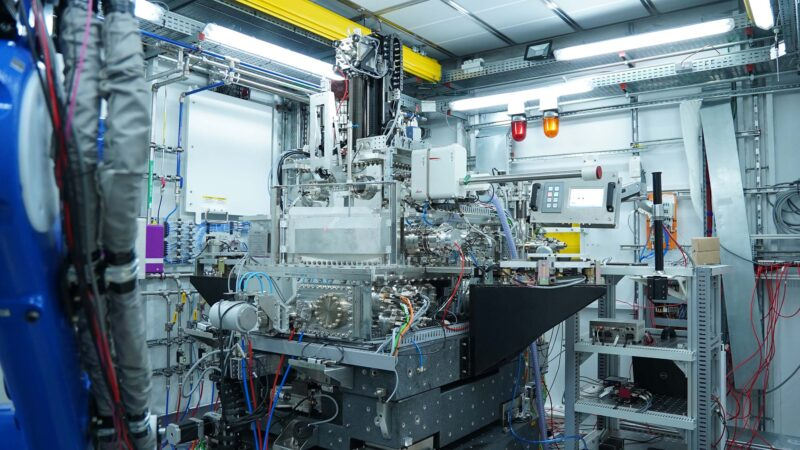
\includegraphics[width=0.9\linewidth]{imagens/SAPOTI.jpg}
    \par\small (a) SAPOTI.
    \par\medskip
    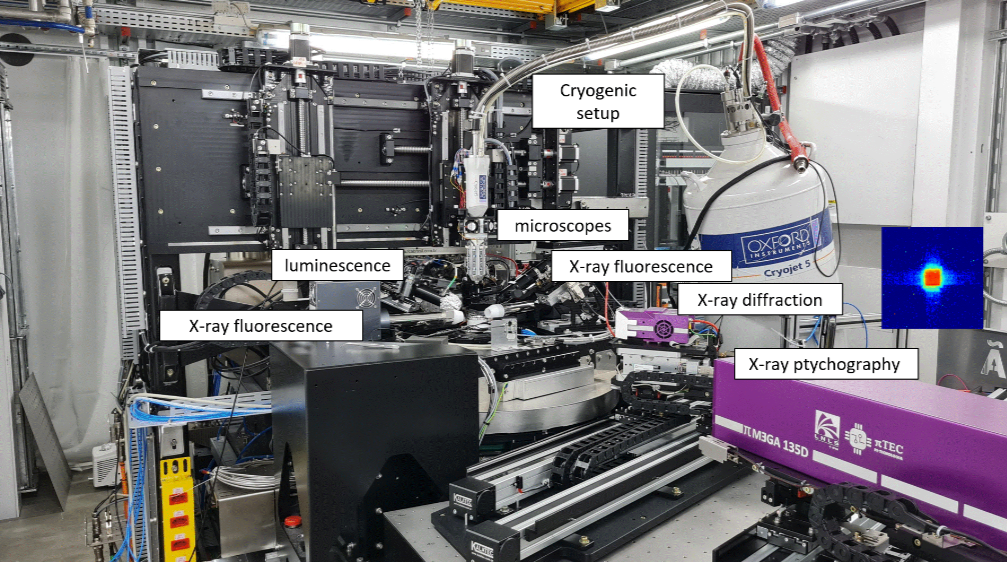
\includegraphics[width=0.9\linewidth]{imagens/TARUMA.png}
    \par\small (b) TARUMÃ.
    \caption{Estações experimentais da linha de luz \CNB: (a) SAPOTI e (b) TARUMÃ.}
    \label{fig:estacoes-sapoti-taruma}
\end{figure}

Destacando agora a funcionalidade dos detectores presentes dentro das estações experimentais para o desenvolvimento do projeto.
Podemos começar com os fotodiodos presentes antes da incidência do feixe sobre a amostra e após a incidência do feixe sobre a amostra, eles são respectivamente chamados de $I_0$ e $I_1$ em referência à equação \ref{eq:absorption-beer-lambert}.
A posição dos fotodiodos e o envio dos sinais para aquisição e armazenamento dos valores de $I_0$ e $I_1$ são ilustrados na Figura~\ref{fig:fotodiodos-aquisicao}.

\begin{figure}[htbp]
    \centering
    \begin{tikzpicture}[x=1cm,y=1cm,>=stealth,font=\small,
        detector/.style={draw,fill=blue!8,minimum width=1.5cm,minimum height=1.6cm,align=center},
        sistema/.style={draw,rounded corners,fill=gray!10,minimum height=1.2cm,align=center}]
        \node[detector] (i0) at (2,0) {Fotodiodo\\$I_0$};
        \node[draw,fill=gray!25,minimum width=1.3cm,minimum height=2cm] (amostra) at (6,0) {Amostra};
        \node[detector] (i1) at (10,0) {Fotodiodo\\$I_1$};
        \draw[->,blue!70!black,line width=2pt] (0,0) -- (i0.west);
        \draw[->,blue!70!black,line width=2pt] (i0.east) -- (amostra.west);
        \draw[->,blue!70!black,line width=0.9pt] (amostra.east) -- (i1.west);
        \node[above] at (0.1,0.4) {Raios-X};
        \node[above,align=center] at (4,0.4) {Feixe\\incidente};
        \node[above,align=center] at (8,0.4) {Feixe\\transmitido};
        \node[sistema,minimum width=4.6cm] (daq) at (6,-3) {Sistema de aquisição\\Leitura dos sinais de $I_0$ e $I_1$};
        \node[sistema,minimum width=4.6cm] (dados) at (6,-5.2) {Armazenamento de dados\\Registros de $I_0$ e $I_1$};
        \draw[->,thick,orange!70!black] (i0.south) -- (2,-3) -- node[above] {Sinal $I_0$} (daq.west);
        \draw[->,thick,orange!70!black] (i1.south) -- (10,-3) -- node[above] {Sinal $I_1$} (daq.east);
        \draw[->,thick] (daq.south) -- node[right] {Valores adquiridos} (dados.north);
    \end{tikzpicture}
    \caption{Diagrama funcional da medição das intensidades incidente e transmitida: o fotodiodo $I_0$ é posicionado antes da amostra e o fotodiodo $I_1$, após a amostra. Os sinais são enviados ao sistema de aquisição, que registra os valores em um sistema de armazenamento de dados. Representação esquemática, sem escala.}
    \label{fig:fotodiodos-aquisicao}
\end{figure}

\phantomsection
\subsection*{Descrição do processamento dos dados experimentais}
\addcontentsline{toc}{subsection}{descrição do processamento dos dados experimentais}

A linha de luz \CNB\ é controlada por um sistema \textbf{EPICS} (\textit{Experimental Physics and Industrial Control System}) que contempla um conjunto de ferramentas \textit{Open-Source} para criação de sistemas distribuídos para controle em tempo real dos instrumentos científicos. \cite{national_Instruments}.

\newpage
\phantomsection
\section*{Resultados}
\addcontentsline{toc}{section}{Resultados}

Nesta seção o autor irá expor o obtido em suas observações. Os resultados poderão estar expressos em quadros, gráficos, tabelas, fotografias ou outros meios que demonstre o que o trabalho permitiu verificar. Os dados expressos não devem ser repetidos em mais de um tipo de ilustração.


\newpage
\phantomsection
\section*{Discussão}
\addcontentsline{toc}{section}{Discussão}

A discussão constitui uma seção com maior liberdade. Nessa fase o autor, ao tempo que justifica os meios que usou para a obtenção dos resultados, pode contrastar esses com os constantes da literatura pertinente.

Na discussão dos resultados o autor deve cumprir as seguintes etapas:

\begin{enumerate}
    \item estabelecer relações entre causas e efeitos;
    \item apontar as generalizações e os princípios básicos;
    \item esclarecer as exceções, modificações e contradições;
    \item indicar as aplicações teóricas ou práticas dos resultados;
    \item elaborar, quando possível, uma teoria para explicar observações;
    \item sugerir, quando for o caso, novas pesquisas.
\end{enumerate}

\newpage
\phantomsection
\section*{Conclusão}
\addcontentsline{toc}{section}{Conclusão}

Mesmo que se tenham várias conclusões deve-se usar sempre o termo no singular, pois, se trata da conclusão do trabalho em si e não um mero enunciado das conclusões a que o(a) autor(a) chegou. É a recapitulação sintética dos resultados e da discussão do estudo ou pesquisa. Pode apresentar deduções lógicas e correspondentes aos objetivos propostos.

\newpage

% ============= REFERÊNCIAS =============

% PASSO 1: Crie um arquivo chamado "referencias.bib" na mesma pasta do seu
%          arquivo .tex e adicione suas fontes no formato BibTeX.
%
%          Exemplo de um livro dentro do arquivo "referencias.bib":
%          @book{SuaChaveUnica1,
%               author    = {Nome do Autor},
%               title     = {Título do Livro},
%               publisher = {Editora},
%               year      = {2025}
%          }

% PASSO 2: No corpo do seu texto, use o comando \cite com a chave única que
%          você definiu no passo 1.
%
%          - Para citação no formato (AUTOR, ANO), use: \cite{SuaChaveUnica1}
%          - Para citação no formato Autor (ANO), use: \citeonline{SuaChaveUnica1}

% As linhas abaixo geram a lista de referências a partir do arquivo .bib
\bibliography{referencias}      % Lê o arquivo "referencias.bib"
\bibliographystyle{abntex2-alf}  % Formata a bibliografia no estilo ABNT (alfabético)

\newpage
% ============= ANEXOS =============
\phantomsection
\section*{Anexos}
\addcontentsline{toc}{section}{Anexos}

Suportes elucidativos e indispensáveis para compreensão do texto são constituídos de documentos, nem sempre elaborados pelo próprio autor, que complementam a intenção comunicativa do trabalho.

\subsection*{ANEXO A -- Questionário}
Conteúdo do anexo A.

\subsection*{ANEXO B -- Representação gráfica}
Conteúdo do anexo B.

\end{document}
